\chapter{Usage Demonstration}~\label{chapter:usage-demo}
This chapter describes three selected demonstrations of the application of the library on practical problems with increasing difficulty: the MAX-ONE problem (Section~\ref{section:maxone}), a self-driving car simulation (Section~\ref{section:self-driving-car}) and an artificial QWOP game player (Section~\ref{section:qwop-player}).

All of the presented examples are included in the attached library distribution package. To ensure that the mentioned results can be replicated, all instances of genetic algorithms use seeded entropy generators.

\section{MAX-ONE Problem}~\label{section:maxone}
The first example is a very trivial problem. It is defined as follows: \textit{Given all bit strings of length between 10 and 55 characters, find the string which maximizes the number of ones.} Although the optimal solution is clearly a string of 55 ones, the simplicity of the problem is ideally suited for a demonstration of the individual components of the library.

The following sections contain a definition of the chromosome data structure and the fitness function for the MAX-ONE problem (Section~\ref{section:maxone-chromosome}), a declaration of the GA itself (Section~\ref{section:maxone-algorithm}) and the results of the algorithm (Section~\ref{section:maxone-results}).

\subsection{Chromosome and Fitness}~\label{section:maxone-chromosome}
The domain space is a finite set. Its points can be characterized as range-initialized arrays of Boolean values with the initialization interval $[10;55]$, which is declared analogically to the array used in solving the Knapsack Problem (see Listing \ref{listing:array-knapsack}). Since range-initialized arrays already support basic genetic operators, they can be used as chromosomes in the GA.

To evaluate and compare the quality of chromosomes, a fitness function is required. For the purposes of this simple example, the fitness function can be defined as
~
\begin{align}
	f(s_1, s_2, \dots, s_{n}) = \frac{1}{55}\sum_{i=1}^{n} s_i
\end{align}
~
where $\{s_i\}_{i=1}^{n}$ are the bits and $n\in[10;55]$ is the length of the chromosome. A simple implementation of a sequential evaluator using this function is shown in Listing \ref{listing:evaluator-sequential-maxone}.

\begin{listing}[ht]
	\inputswift{evaluator-sequential-maxone}
	\caption{Example of a sequential evaluator for the MAX-ONE Problem.}
	\label{listing:evaluator-sequential-maxone}
\end{listing}

\subsection{Algorithm}~\label{section:maxone-algorithm}
With both the chromosome data structure and the fitness function defined, the only remaining step is to declare and configure the instance of the GA before a run can be started. 

\begin{listing}[ht]
	\inputswift{algorithm-maxone}
	\caption{Example of the GA definition for the MAX-ONE Problem.}
	\label{listing:algorithm-maxone}
\end{listing}

To clearly explain the syntax of the \texttt{GeneticAlgorithm<T>} class initializer, the algorithm shown in Listing \ref{listing:algorithm-maxone} has the following properties:
~
\begin{itemize}
	\item The number of individuals in every generation is 200.
	\item Elitism is used to preserve the best chromosome.
	\item The algorithm terminates after 1000 iterations or after the highest fitness value reaches 1.0.
	\item The $\beta$-tree contains a single chance node:
	~
	\begin{itemize}
		\item With the probability 0.5, apply the reproduction operator on a random individual.
		\item With the probability 0.3, apply the mutation operator on an individual selected by the roulette selection.
		\item With the probability 0.2, apply the one-point crossover operator on the winners of two randomized tournaments, each containing five contestants.
	\end{itemize}
\end{itemize}

\subsection{Results}~\label{section:maxone-results}
When executed, the presented algorithm performs 270~iterations before reaching the best fitness value~1.0 and yielding the optimal solution consisting of 55~ones. On the experimental computer\footnote{The experimental computer was Apple Mac mini (model \textit{Late 2012}) with Intel Core i7 CPU (2.3~GHz) and 8~GB RAM (1600~MHz DDR3).}, the evaluation of the algorithm took approximately 1.55~seconds.

To further increase its speed, it is possible to utilize parallelization of fitness evaluation as described in Section \ref{section:parallel-evaluators}. By substituting the line no. 13 of Listing \ref{listing:algorithm-maxone} with \mintinline{swift}{ParallelEvaluator() { _ in MaxOneEvaluator() }}, the library creates a separate evaluator instance for every CPU core, instead of sharing a single instance among all cores.

After this modification, the number of performed iterations remains the same, however, the total execution time decreases to 1.46~seconds. Note even though the experimental computer has 8 core CPU, such a small decrease in evaluation time is acceptable due to the fact that the only parallelized part of the algorithm is the evaluation of the fitness function, which in this particular case does not represent a significant portion of the processing time. The convergence of fitness values is plotted in Figure \ref{fig:maxone-fitness}.

\begin{figure}[ht]
	\centering
	\begin{tikzpicture}
		\begin{axis}[
			height=9cm,
			width=0.9\textwidth,
			grid=major,
			xlabel={Generation},
			ylabel={Fitness},
			ymin=0, ymax=1,
			xmin=1, xmax=270,
			no markers,
			legend pos=south east
		]
			
		\addplot table {data/maxone-fitness-best.dat};
		\addlegendentry{Best fitness}

		\addplot table {data/maxone-fitness-average.dat};
		\addlegendentry{Average fitness}

		\end{axis}
	\end{tikzpicture}
	\caption[MAX-ONE genetic algorithm fitness convergence chart.]{Fitness convergence chart of the GA from Listing \ref{listing:algorithm-maxone}.}
	\label{fig:maxone-fitness}
\end{figure}

\section{Self-driving Car Simulation}~\label{section:self-driving-car}
The second example can be considered slightly more complex and closer to practical applications than the MAX-ONE Problem. Suppose that there is a robot car capable of navigating in a simulated two-dimensional environment (illustrated by Figure \ref{fig:self-driving-car}) which contains a closed curve resembling a \textit{race track}. The objective is to find a way to steer the car, so that it discovers the track and follows its contour. In real-world applications, this objective would be an analogy to keeping a car or a car-like drone within the bounds of a marked road.

\begin{figure}[ht]
	\centering
	\begin{tikzpicture}[framed,background rectangle/.style={draw,fill=black!60!green}]
		\draw[
		  black!10!white,
		  line width=3mm,
		  postaction={
		    decorate,
		    decoration={
		      markings,
		      mark=between positions 0 and 1 step 0.2 with
		      {
		        \node[transform shape] {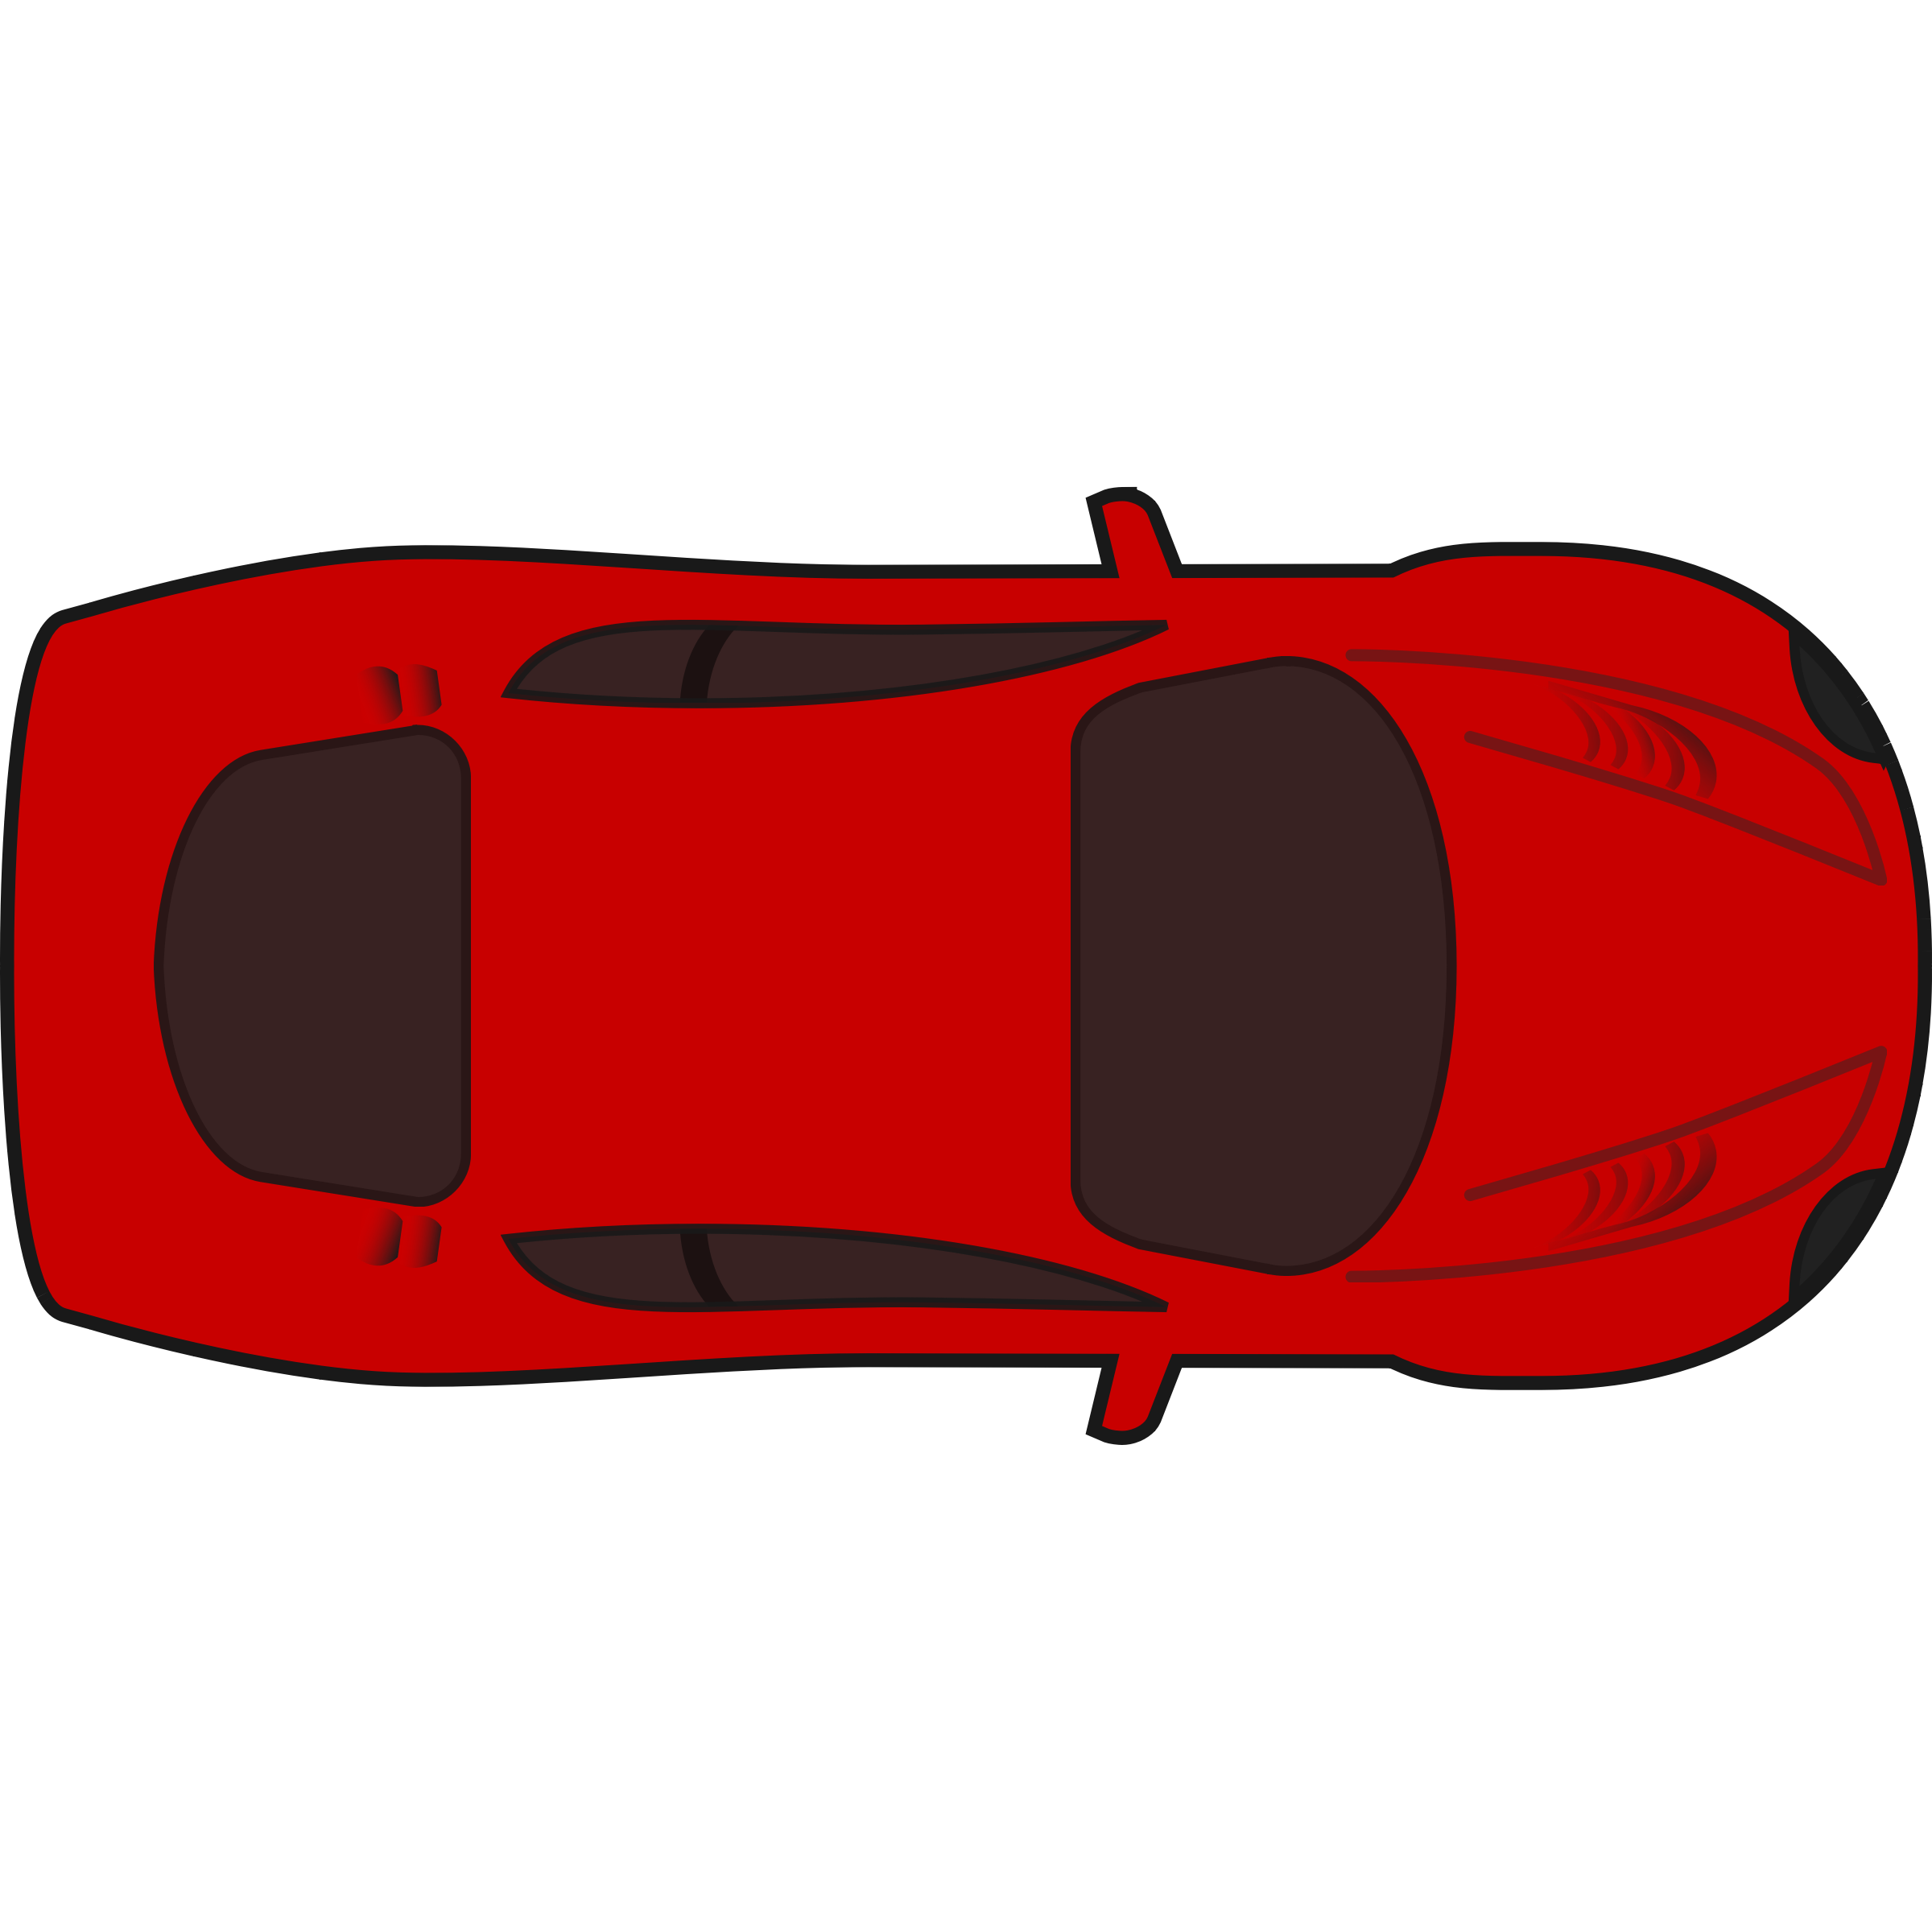
\includegraphics[width=.5cm]{img/car}};
		      }
		    }
		  }
		]
		(0,0) to[out angle=0,in angle=180,curve through={(1,.4) .. (5,0) .. (10,.5) .. (7,4.3) .. (3,4) .. (1,2)}] (0,0);
	\end{tikzpicture}
	\caption{Illustration of the self-driving car simulation environment.}
	\label{fig:self-driving-car}
\end{figure}

The simulated car is controlled by two parameters: the \textit{steering} and the \textit{acceleration}. Modelled after physical driving control systems like the steering wheel and the accelerator pedal, changes in these parameters cannot influence the heading and the velocity of the car directly. Instead, the control parameters affect car's heading and velocity gradually with respect to the time, behaving more like their first derivatives.

An event loop operates in the simulated environment, evaluating all variables periodically with a sufficient\footnote{For the experiments, the frequency of the event loop has been set to 40 Hz.} frequency. This event loop is responsible for periodically altering the position of the car with respect to its instantaneous velocity and recalculating the instantaneous velocity with respect to the latest value of the acceleration control parameter. A similar process serves to adjust the heading of the car. However, while the acceleration is a continuous decimal parameter with values chosen within a set interval, the steering parameter is fundamentally different, being a discrete choice between set values:
~
\begin{description}
	\item[Hard left]
	Alter heading by $+\frac{1}{2}\pi$ radians with respect to the driver's viewport.

	\item[Left]
	Alter heading by $+\frac{1}{4}\pi$ radians with respect to the driver's viewport.

	\item[Neutral]
	Maintain current heading.

	\item[Right]
	Alter heading by $-\frac{1}{4}\pi$ radians with respect to the driver's viewport.

	\item[Hard right]
	Alter heading by $-\frac{1}{2}\pi$ radians with respect to the driver's viewport.
\end{description}

To recognize the race track in the environment, the robotic car is equipped with a set of simulated real-time detectors, which are positioned in a way to approximate the viewport of a real car driver. There are three detectors located in front of the car, one under the car and one behind it. All detectors are capable of producing Boolean values, signifying whether the track is located on their exact position at the time of measurement. This configuration approximates thresholding techniques frequently used in detectors of real self-driving car prototypes.

In all simulations, the environment has square shape with the side equal to 10 kilometers. If at any point throughout the simulation the center of the car leaves the bounds of the environment, the simulation terminates. The simulation also ends if set maximum duration is exceeded. The simulated properties of the car (such as dimensions, maximum acceleration, etc.) mimic\footnote{The simulation limits the acceleration and the instantaneous velocity of the car to match the capabilities of its real-world equivalent. However, it is worth noting that the restrictions are exerted unrealistically by clamping numerical values.} those of \textit{Audi R8 5.2 V10 FSI Quattro (model 2010)}.

The race track is non-deterministically generated at the beginning of the simulation. First, 30 to 50 points are chosen within the environment at random. These points are in fact selected from a slightly smaller padded rectangle within the environment bounds in order to prevent the generated track from accidentally leading the car to the edges of the environment. In the next step, the convex hull of the selected set of points is calculated by the Melkman Algorithm. \cite{MelkmanConvexHull} The points of the convex hull are transformed to a Bézier curve by simple interpolation utilizing cubic Catmull-Rom splines. \cite{CatmullRomSplines} Lastly, the thickness of the track curve is increased to 5 meters in order to improve tolerance in subsequent hit-testing.

In the following sections, the control program of the car (Section~\ref{section:car-control-program}), the chromosome data structure and the fitness function (Section~\ref{section:car-chromosome}) are defined. The GA is described in Section~\ref{section:car-algorithm} and its results are discussed in Section~\ref{section:car-results}.

\subsection{Control Program}~\label{section:car-control-program}
The control program of the car is a dedicated real-time software, which periodically interacts with the event loop of the environment in order to determine the values of control parameters based on the outputs of the on-board detectors.

To demonstrate how the presented library can be used in conjunction with other Swift components, it was decided that the car is to be controlled by a three-layer feedforward neural network with common sigmoid activation function (for definition, see Section \ref{section:neural-networks}). The input layer of the network is comprised of 5 nodes corresponding to binary read-outs of the on-board detectors, the hidden layer contains 10 nodes and the output layer contains 2 nodes which correspond to the control parameters of the car.

While the acceleration parameter is directly equal\footnote{The acceleration parameter is artificially limited to better approximate physical limitations of the car.} to the output of its respective node, the steering parameter uses thresholds to determine the change in heading.

\subsection{Chromosome and Fitness}~\label{section:car-chromosome}
It is possible to encode the neural network described in the previous section as a real vector from $d$-dimensional space, where $d$ denotes the number of interunit connections and the components of the vector correspond to weight coefficients of such connections. By assuming that all connections between nodes from consecutive layers exist (substituting the weight 0 for non-existing connections), a fixed length of the vector can be ensured. The neural network can thus be characterized by a range-initialized array of real numbers with the initialization interval $[d;d]$. Accounting for 5, 10 and 2 nodes in the input, hidden and output layer respectively along with the bias parameters, $d=6\cdot 10+11\cdot 2=82$.

To evaluate and compare the quality of control programs, a simple simulated test is performed. Prior to the test, a random race track is generated and positioned within the environment. The car is placed in the center of the simulation with random heading and velocity. Since the race track is a closed curve, the car's initial straight-line trajectory intersects it in at least one point. The control program of the car is expected not to interfere significantly with the steering of the car up to this point. However, after reaching it, the control program should take action to prevent the car from leaving the track.

The described test scenario is executed multiple times, in each instance with different random initial conditions. Throughout every test, various parameters of the car are monitored and recorded by the event loop of the simulation. Every test is terminated if one of two conditions is satisfied:
~
\begin{enumerate}
	\item the center point of the car leaves the bounds of the environment, or
	\item the maximum duration of the simulation (1 hour) is exceeded.
\end{enumerate}

A crucial parameter for the calculation of fitness values is the \textit{total distance driven over the race track} (denoted $\hat{d}$). Upon initialization, the distance is set to zero. In every iteration of the event loop, the traveled distance $\Delta d$ is calculated from the instantaneous velocity and the event loop frequency. If the detector located in the middle of the car reports contact with the race track, the calculated distance $\Delta d$ is added to $\hat{d}$, otherwise $\hat{d}$ remains unchanged. Clearly, $\hat{d}$ has only nonnegative values. For the purposes of the simulation, $\hat{d}$ has an upper bound in the distance traveled at the highest allowed velocity for the maximum duration of the simulation, which is $d_{max}=199,980$ m/s. At this point, the fitness function can be defined. The fitness function of the control program is evaluated as
~
\begin{align}
	f(\hat{d}_1,\hat{d}_2,\dots,\hat{d}_5) = \frac{1}{5 \cdot d_{max}} \sum_{i=1}^5 \hat{d}_i
\end{align}
~
where $\hat{d}_1,\hat{d}_2,\dots,\hat{d}_5$ denote the total distances driven over the race track calculated in tests 1 through 5 respectively. All distances are specified in meters.

Clearly, the presented fitness function favors control programs which manage to keep the car on the track more than programs which do not follow it very well or veer off it eventually. In addition, since the function operates on distances, control programs are motivated to discover the race track as quickly as possible and to maximize the distance traveled over it. An implementation of a sequential evaluator using this function is illustrated in Listing \ref{listing:evaluator-sequential-car}.

\begin{listing}[ht]
	\inputswift{evaluator-sequential-car}
	\caption{Implementation of the self-driving car evaluator.}
	\label{listing:evaluator-sequential-car}
\end{listing}

In the evaluator, the control program along with the neural network itself\footnote{The implementation of the FFNN was provided by the \textit{Swift AI} open-source project, which is available online: \url{https://github.com/collinhundley/Swift-AI}} is encapsulated in an instance of the \texttt{NetDriver} type, which is conformant to the \texttt{CarDriver} protocol that formalizes requirements on automated car controllers (not necessarily only those operating with neural networks). Since the evaluator is fully self-contained, it enables parallelization by \texttt{ParallelEvaluator<T>} which was shown in the last example. To visualize the simulation, the \texttt{CarSimulation} initializer can be called in the \textit{verbose}, which automatically generates a MATLAB script capable of displaying animated plot of the car's position in time.

\subsection{Algorithm}~\label{section:car-algorithm}
The GA declaration is analogous to that used in the MAX-ONE Problem (see Listing \ref{listing:algorithm-maxone}). The GA has been configured with the following properties:
~
\begin{itemize}
	\item The number of individuals in every generation is 200.
	\item Elitism is used to preserve the best chromosome.
	\item The algorithm terminates after 100 iterations are performed or after the highest fitness value reaches 1.0.
	\item The $\beta$-tree contains a single chance node:
	~
	\begin{itemize}
		\item With the probability 0.8, apply the reproduction operator on a random individual.
		\item With the probability 0.8, apply the mutation operator on an individual selected by the roulette selection.
		\item With the probability 0.1, apply the one-point crossover operator on the winners of two randomized tournaments, each containing five contestants.
	\end{itemize}
\end{itemize}

\subsection{Results}~\label{section:car-results}
When executed, the presented algorithm performs 100~iterations, reaching the best fitness value~0.973. Unlike the MAX-ONE algorithm, the convergence rate of the execution is quite high, possibly hinting at suboptimal solution. On the experimental computer\footnote{The experimental computer was Apple Mac mini (model \textit{Late 2012}) with Intel Core i7 CPU (2.3~GHz) and 8~GB RAM (1600~MHz DDR3).}, the evaluation of the algorithm took approximately 4.2~hours with the parallelization enabled. The convergence of fitness values is plotted in Figure \ref{fig:car-fitness}.

\begin{figure}[ht]
	\centering
	\begin{tikzpicture}
		\begin{axis}[
			height=9cm,
			width=0.9\textwidth,
			grid=major,
			xlabel={Generation},
			ylabel={Fitness},
			ymin=0, ymax=1,
			xmin=1, xmax=100,
			no markers,
			legend pos=south east
		]
			
		\addplot table {data/car-fitness-best.dat};
		\addlegendentry{Best fitness}

		\addplot table {data/car-fitness-average.dat};
		\addlegendentry{Average fitness}

		\end{axis}
	\end{tikzpicture}
	\caption{Fitness convergence chart of the self-driving car GA.}
	\label{fig:car-fitness}
\end{figure}

\section{Artificial QWOP Player}~\label{section:qwop-player}
The third and final usage demonstration of the presented library is closely related to genetic programming techniques shown in \cite{EvolvingQwopGaits}.

In the cited literature, researchers describe their attempts at training artificial programs in playing an online computer game, achieving scores comparable to or exceeding those of human players. This section is dedicated to replicating parts of their results.

In the following sections, the QWOP game is described in detail (Section~\ref{section:qwop-description}) as well as the previous works related to it (Section~\ref{section:qwop-previous-work}). Section~\ref{section:qwop-interface} gives details on the technical caveats of interfacing an existing Java application with the GA programmed in Swift. Lastly, the GA is defined (Section~\ref{section:qwop-algorithm}) and its results are discussed (Section~\ref{section:qwop-results}).

\subsection{The QWOP Game}~\label{section:qwop-description}
QWOP (shown in Figure \ref{figure:QWOP}) is a popular online game, available for free at Foddy.net \cite{QwopWebsite}. In the game, the player controls movements of an Olympic athlete during a sprint race. The objective is to reach the longest possible distance, terminating at the 100-meter mark. If at any point throughout the race, the head or any of the hands of the athlete come into contact with the ground, the athlete loses his balance, falls and the game is over. The control scheme of QWOP is very simple. By pressing keys Q, W, O, P on the keyboard (hence the name of the game), the player controls movements of different muscle groups within the athlete's body. Keys Q and W move forward the left and the right thighs and keys O and P move backward the left and the right calves respectively.

\begin{figure}[ht]
	\centering
	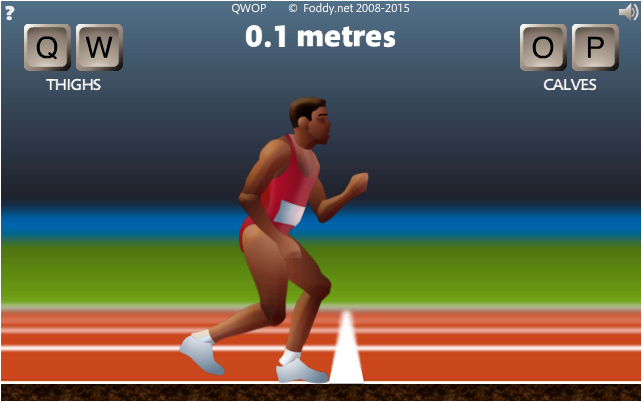
\includegraphics[width=0.8\textwidth]{img/qwop.png}
	\caption[The QWOP online game.]{The QWOP online game. \cite{QwopWebsite}}
	\label{figure:QWOP}
\end{figure}

In spite of the simplicity of the game goals and its straightforward control scheme, QWOP is well-known for its notorious difficulty. This is mainly due to its ``ragdoll physics'' engine, which heavily oversimplifies the mechanics of the simulated runner to the point where certain behaviors might seem unintuitive or even unpredictable. \cite{QwopHomework} The biggest challenge of the game can be described as to devise a repeatable strategy to achieve and maintain precise synchronization of key presses, receiving only limited sensory feedback from the game.

\subsection{Previous Work}~\label{section:qwop-previous-work}
QWOP has been previously mentioned in several publications, mostly in relation to machine learning. The challenge of the game has been subject of study primarily because of its appearent similarity to the problem of evolving bipedal gaits in physical robots and other cybernetic applications.

To describe QWOP strategies, the authors of \cite{EvolvingQwopGaits} have used string encodings. Since one of these encodings is used\footnote{The used encoding is the \textit{Encoding 1}, which was originally proposed by \cite{QwopEncoding}.} in this demonstration, its definition is included in this section. The encoded strings represent sequences of instructions to the player without any regards to the state of the game. The encoding uses symbols ``\texttt{q,Q,w,W,o,O,p,P,+}''. A capital letter represents pressing the corresponding key on the keyboard, a lowercase letter represents a key release. The ``\texttt{+}'' symbol stands for a delay in which the current state of inputs is maintained for 150 milliseconds. \cite{EvolvingQwopGaits}

Upon interpretation, the encoded string is read from the left to the right, executing one instruction at a time. When the end of the string is reached, the interpretation starts again from the beginning. An example of a strategy encoded in this way is shown in Listing \ref{listing:encoding-example}.

\begin{listing}[ht]
	\begin{minted}[frame=lines,
               framesep=2mm,
               fontsize=\small]{text}
QO+qPW+wpo+QPW+wO+qp+P+Q+++qp+QPW+wo+qp+POQ+q+W+Qp+qwo
	\end{minted}
	\caption[Example encoded QWOP game strategy.]{Example encoded QWOP game strategy, which translates to \textit{``Press Q and O, hold them for 150 ms, release Q, press P and W, hold for 150 ms, release W, P and O, wait...''} \cite{EvolvingQwopGaits}}
	\label{listing:encoding-example}
\end{listing}

To consistently interpret QWOP strategies encoded into strings, the authors of \cite{EvolvingQwopGaits} have used automated Java program called the \textit{Qwopper}, which has been originally developed by \cite{QwopEncoding}. The application is comprised of three components:
~
\begin{description}
	\item[Strategy interpretter]
	The interpretter is responsible for creating artificial user inputs for the QWOP game in compliance with a given strategy string.

	\item[Control interface]
	The control interface is a user application, which serves users to configure and test the interpretter.

	\item[GA engine]
	By default, Qwopper includes its own implementation of the GA, which has been used to produce strings by means of genetic programming.
\end{description}

Apart from blindly simulating user inputs, the interpreter component of Qwopper includes a basic OCR algorithm (illustrated in Figure \ref{figure:QWOP-OCR}), which is capable of determining the current state of the game (\textit{running} or \textit{paused}) and reading the distance traveled by the athlete. Combining this information with the duration of the run, Qwopper can periodically estimate the instantaneous velocity of the runner achieved by a given strategy.

\begin{figure}[ht]
	\centering
	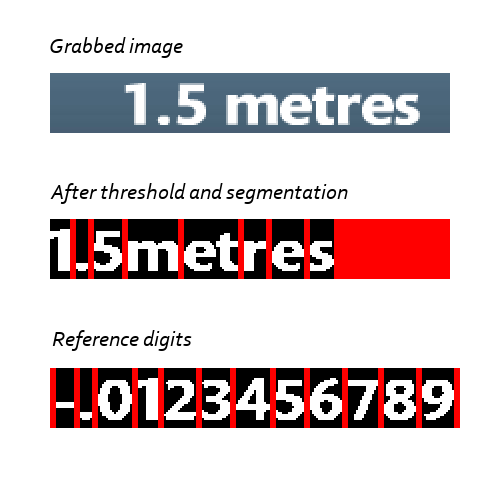
\includegraphics[width=0.5\textwidth]{img/reading_digits.png}
	\caption[OCR process used by the Qwopper software.]{Illustration of the OCR process used by the Qwopper software. \cite{QwopEncoding}}
	\label{figure:QWOP-OCR}
\end{figure}

It is worth noting at this point that Qwopper already has all necessary components to generate, evaluate and recombine QWOP strategy strings on its own. However, for the purpose of demonstration of the GA provided by the presented library, its functions are reduced to only serve as a strategy string evaluation tool.

\subsection{Interfacing Qwopper with Swift}~\label{section:qwop-interface}
The encoding defined in the previous section can be simply used in a chromosome data structure. By the use of Swift enumerations and the conformance to the \texttt{Discrete} protocol (for usage example, see Listing \ref{listing:discrete-sample}), QWOP game strategies can be stored in a range-initialized array with the initialization interval $[1;200]$.

To efficiently evaluate different game strategies, it is imperative that the Qwopper application is capable of communicating with the GA implemented in Swift. For that reason, the main interface of Qwopper has been altered to serve this purpose. Upon execution, the modified version of Qwopper receives three shell parameters:
~
\begin{description}
	\item[Strategy string]
	The strategy to evaluate. For example, see Listing \ref{listing:encoding-example}.

	\item[Number of attempts]
	How many times should the runs be repeated.

	\item[Maximum duration]
	The maximum duration of a single run in milliseconds.
\end{description}

After parsing the input, the application finds an open game window and attempts to play the game, following the instructions in the strategy string. When the athlete falls or the set maximum duration is exceeded, the application prints information about the run to the standard output and starts another run (or terminates). The monitored information includes:
~
\begin{description}
	\item[Result]
	A Boolean flag signifying whether the athlete has fallen in the run.

	\item[Duration]
	Duration of the run in milliseconds.

	\item[Distance]
	Distance achieved by the athlete in meters.
\end{description}

In the evaluation of the GA, the execution of Qwopper is represented by a \texttt{QwopEvaluator} object, which is a subclass of the \texttt{SequentialEvaluator<T>} type. This object is responsible for executing the application with correct parameters and reading its outputs, from which the value of the fitness function is calculated. The fitness function of a QWOP strategy is defined as
~
\begin{align}
	f(d_1,d_2,\dots,d_n) = \frac{1}{n \cdot d_{max}} \sum_{i=1}^n d_i
\end{align}
~
where $d_1,d_2,\dots,d_n$ denote the distances run by the athlete in $n$ individual attempts at executing the strategy by Qwopper. The value $d_{max}=100$ is the maximum achievable distance of a single run. All distances are specified in meters. Since multiple active instances of Qwopper could interfere with each other, instances of the \texttt{QwopEvaluator} type do not support parallelization of fitness evaluation shown in the previous demonstrations.

\subsection{Algorithm}~\label{section:qwop-algorithm}
Due to the time-consuming nature of fitness evaluation and the lack of parallelization options, the GA for the QWOP runner training has been configured with the following parameters:
~
\begin{itemize}
	\item The number of individuals in every generation is 80.
	\item Elitism is used to preserve the best chromosome.
	\item The algorithm terminates after 18 hours of execution or after the highest fitness value reaches 0.8.
	\item In the evaluation of a single strategy, Qwopper attempts 1 run with the maximum duration of 30 seconds.
	\item The $\beta$-tree contains a single chance node:
	~
	\begin{itemize}
		\item With the probability 0.5, apply the reproduction operator on a random individual.
		\item With the probability 0.3, apply the mutation operator on an individual selected by the roulette selection.
		\item With the probability 0.2, apply the one-point crossover operator on the winners of two randomized tournaments, each containing five contestants.
	\end{itemize}
\end{itemize}

\subsection{Results}~\label{section:qwop-results}
When executed, the presented algorithm performs 38~iterations, reaching the best fitness value~0.224. On the experimental computer\footnote{The experimental computer was Apple Mac mini (model \textit{Late 2012}) with Intel Core i7 CPU (2.3~GHz) and 8~GB RAM (1600~MHz DDR3).}, the evaluation of the algorithm took approximately 18~hours. The convergence of fitness values is plotted in Figure \ref{fig:qwop-fitness}.

\begin{figure}[ht]
	\centering
	\begin{tikzpicture}
		\begin{axis}[
			height=9cm,
			width=0.9\textwidth,
			grid=major,
			xlabel={Generation},
			ylabel={Fitness},
			ymin=0, ymax=0.4,
			xmin=1, xmax=38,
			no markers,
			legend pos=north east,
			ytick={0.1,0.2,...,0.4}
		]
			
		\addplot table {data/qwop-fitness-best.dat};
		\addlegendentry{Best fitness}

		\addplot table {data/qwop-fitness-average.dat};
		\addlegendentry{Average fitness}

		\end{axis}
	\end{tikzpicture}
	\caption{Fitness convergence chart of the QWOP GA.}
	\label{fig:qwop-fitness}
\end{figure}

The best strategy of the last generation (shown in Listing \ref{listing:best-strategy}) was capable of controlling the athlete successfully, finishing the 100-meter race in approximately 152 seconds. This result is comparable with those presented in \cite{EvolvingQwopGaits}, where the authors state that one of the best-evolved gaits which used the same encoding achieved the same distance in ``about 2 minutes.''

\begin{listing}[ht]
	\begin{minted}[frame=lines,
               framesep=2mm,
               fontsize=\small]{text}
oQqpqQWWPqQqWoOwqOqoPpQOwPWo+oowOqWqwWqwOp+qoPOwpoWWOQwowqW+WOP+qqwpo+Qq
wpqPwp
	\end{minted}
	\caption[The best discovered QWOP game strategy.]{The best discovered QWOP game strategy (fitness 0.224).}
	\label{listing:best-strategy}
\end{listing}
